\documentclass[dvips, 12pt]{article}

% Any percent sign marks a comment to the end of the line

% Every latex document starts with a documentclass declaration like this
% The option dvips allows for graphics, 12pt is the font size, and article
%   is the style


\usepackage[margin=1in]{geometry}

\usepackage{graphicx}
\usepackage{url}
\usepackage{harmony}
\usepackage{musixtex}
\usepackage{subfigure}
\usepackage{caption}
%\usepackage{biblatex}
%\usepackage{subcaption}

% These are additional packages for "pdflatex", graphics, and to include
% hyperlinks inside a document.


% These force using more of the margins that is the default style


% Everything after this becomes content
% Replace the text between curly brackets with your own

\title{{\Huge \bfseries SMURF} \\ \Large \it Serial MUsic Represented as Functions \vspace{0.6cm}}

\author{\normalsize Richard Townsend, Lianne Lairmore, Lindsay Neubauer, Van Bui, Kuangya Zhai
	\\ \small \{rt2515, lel2143, lan2135, vb2363, kz2219\}@columbia.edu \vspace{0.6cm}}

\date{\today \vspace{2cm}}

% You can leave out "date" and it will be added automatically for today
% You can change the "\today" date to any text you like

\begin{document}
\maketitle


% This command causes the title to be created in the document

SMURF is a functional language that will allow a composer to create serialist music
based on twelve-tone composition. In general, serialism is a musical composition
technique where a set of values, chosen through some methodical process, generates
a sequence of musical elements. Our languge will be based on the functional syntax
and semantics set forth by Haskell, and we will compile our programs into C.
The C program will then use openGL to generate images of sheet music corresponding to the user's
initial program in SMURF.

\section{Background: What is Serialism?}

In general, serialism is a musical composition technique where a set of values, chosen through some methodical process, 
generates a sequence of musical elements. Its origins are often attributed to Arnold Schoenberg's twelve-tone technique, which
he began to use in the 1920s. In this system, each note in the chromatic scale is assigned an integer value, giving us a set of twelve
``pitch classes'' (Figure~\ref{fig:pc}).
A composer utilizing this method then takes each of these integers, and orders them into a $twelve$ $tone$ $row$, where 
each number appears exactly once. We refer to this row as the $prime form$ of a piece, and conventionally refer 
to it as $P_0$. 

\begin{figure}
\begin{minipage}{0.6\textwidth}
	\centering
	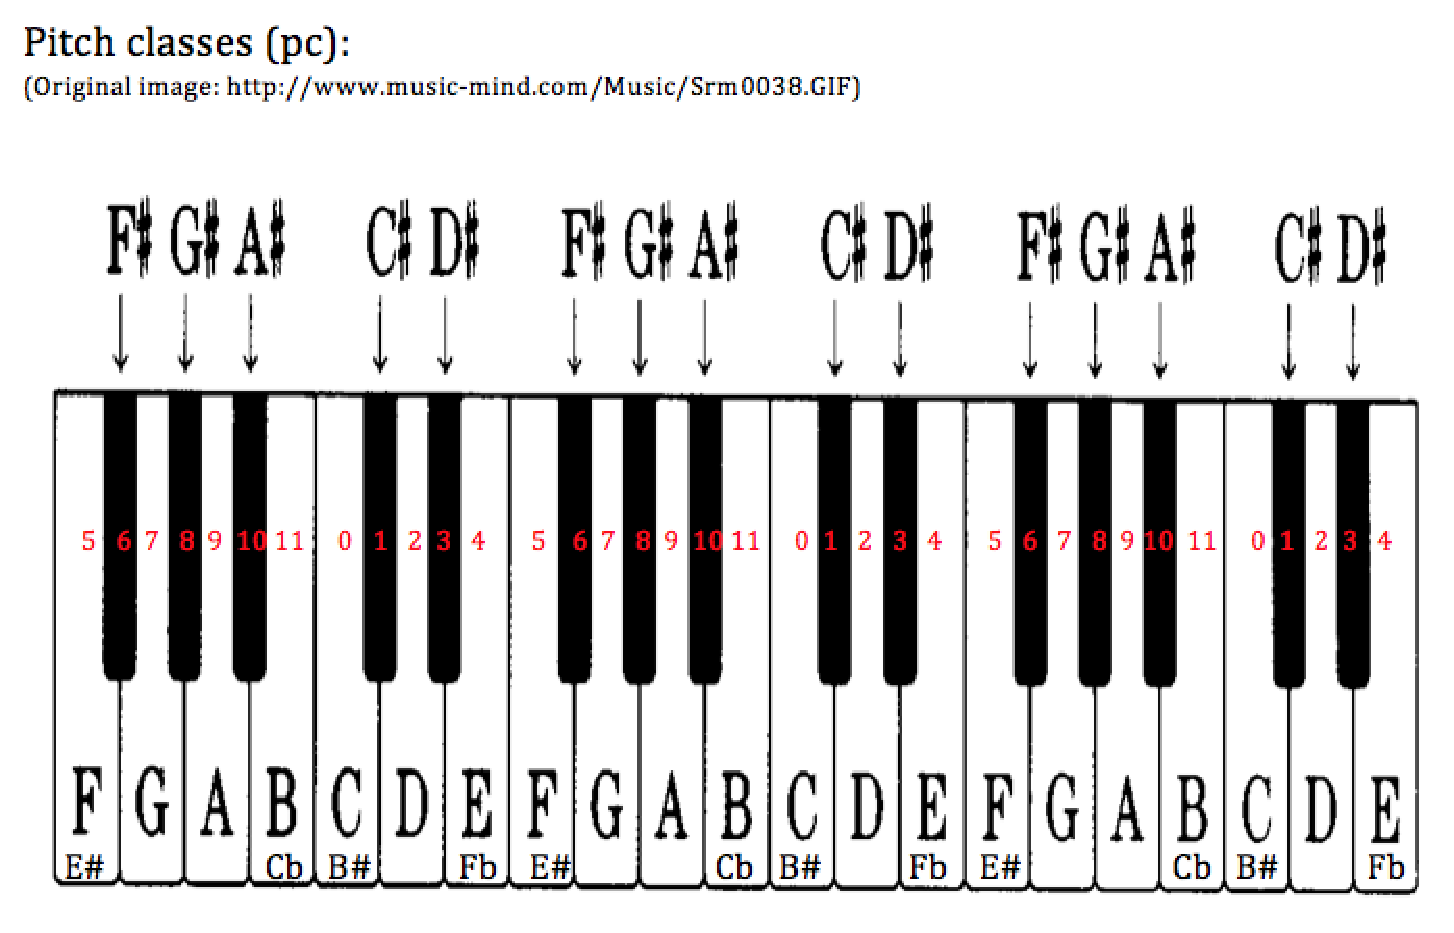
\includegraphics[width=\textwidth]{figures/serialismPianoImage}
	\caption{pitch classes}
	\label{fig:pc}
\end{minipage}\hfill
\begin{minipage}{0.4\textwidth}
	\centering
		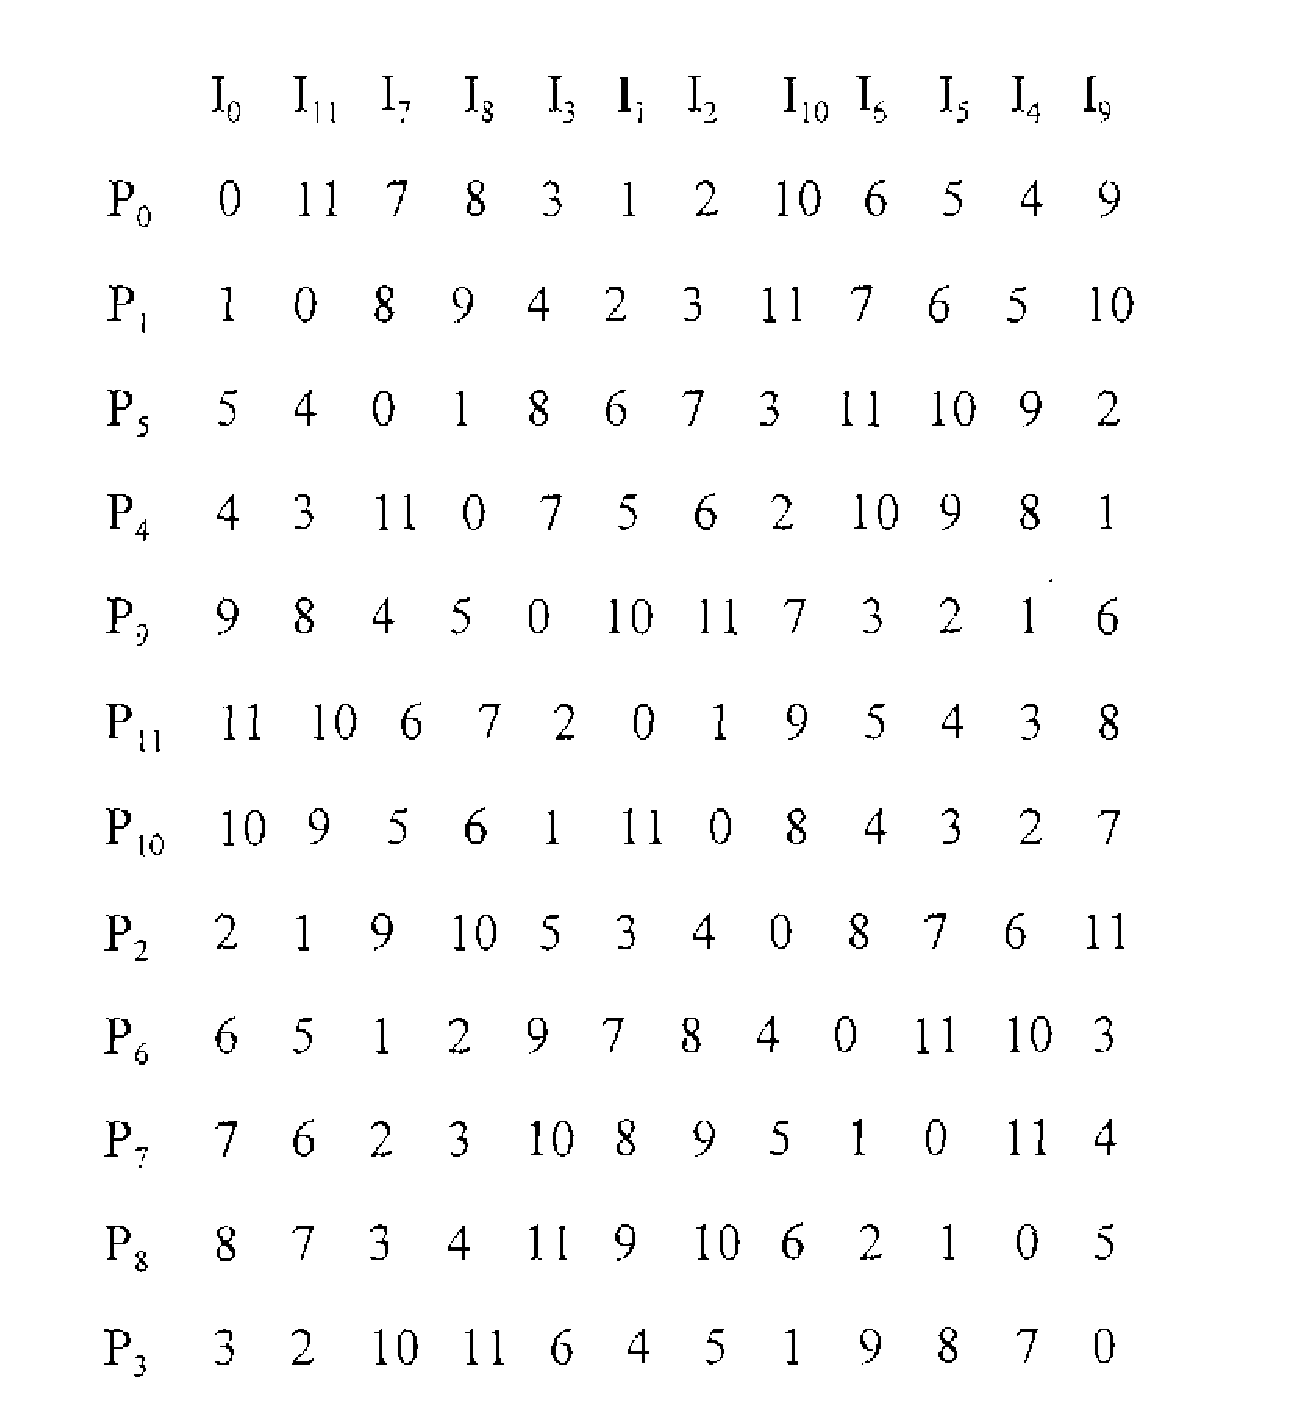
\includegraphics[width=\textwidth]{figures/12_tone}
	\caption{twelve tone matrix}
	\label{fig:12tone}
\end{minipage}
\end{figure}


The composer can then generate other rows that are derived from $P_0$ through three types of transformations:
transposition, inversion, and retrograde. In each of these transformations, we always use mod 12 arithmetic to preserve the 
numbering system of our pitch classes. Transposing a row consists of taking each pitch class in the row and adding the same number 
to each. If we transpose $P_0$ by four semitones, we add four mod twelve to each pitch class in $P_0$ and end up with a new row 
called $P_4$. In general, $P_x$ is a transposition of $P_0$ by $x$ semitones. To invert a row, we flip each interval between two 
pitch classes in that row. For example, if $P_0$ starts with pitch classes 0-4-1, then we have an interval of +4 between the first two 
pitches and -3 between the second two. In the inverse of $P_0$ (called $I_0$), the first interval would be -4 and the second would 
be +3, giving us 0-8-11 as our first three pitch classes. The subscript of $I_x$  refers both to the number of transpositions required 
to arrive at $I_x$ from $I_0$, and to the prime row $P_x$ that would need to be inverted to generate $I_x$. The final row 
operation is a retrograde transformation, which merely consists of reading a row backwards. That is, $R_x$ is generated by reading 
the pitch classes of $P_x$ in their opposite order. One can also have a retrograde inversion; $RI_x$ is generated by reading the 
pitch classes of $I_x$ backwards.

Once a composer chooses a $P_0$, the three transformations outlined above can be applied to varying degrees to generate a $twelve$ $tone$ $matrix$, which will contain each $P$ row as a row in the matrix and each $I$ row as a column.
Furthermore, all of the $R$ and $RI$ rows are found by reading the rows in the matrix from right to left or the columns 
from bottom to top, respectively. An example of a 
twelve tone matrix from one of Shoenberg's pieces can be found in Figure~\ref{fig:12tone}. Finally, using the twelve tone matrix as a guide,
	   the composer picks various rows and columns to serve as melodic and harmonic elements in their composition, resulting in a piece
	   of serial music.
	   %Possible transformations
	   %Notation


\section{Motivation}

Our group has decided to create a language that will assist a composer in creating music 
using the twelve tone method described above. We plan on making this language 
functional and compile into C. The compilation process will create a C program 
that will use openGL to create an image representing the music created. 

Twelve tone serialism is a mathematically intensive method of creating music which 
involves mapping notes to numbers. It is very natural to work with twelve tone rows 
using a programming language since the method just treats notes like numbers that 
can be added and subtracted from. We plan on our language making twelve tone compilation 
easier using data types and functions specifically for the purpose of creating music in 
this way. By simplifying the method of inverting and transposing rows composers can focus 
more on how to exploit new ways to make music in this fashion and worry less about 
creating matrices. 

We chose to implement our language as a functional language because of the clear and 
succinct programs that functional languages produce. It also makes sense for our language 
to be functional because functional languages also are well known for their ability to 
work on lists and most arithmetic done in twelve tone serialism is done on rows or 
columns. As a group we are also very interested on how a functional language compiler 
works. 

Instead of compiling our language into byte code which can be interpreted and play the 
notes we thought it would be more interesting to create a language that could be compiled 
into a score. Scores are made up of just lines and dots and would be easy to create in 
a graphics library like openGL. We decided to compile our language into C since it was a 
significantly less abstract language which had access to openGL library calls. One benefit 
of compiling into C and not a language to be interpreted as music is that programs in our 
language could be created that do not actually output any music but instead create 
functions that could be used in other programs to do the same transformation of rows. 
That way our language is not just limited to functions defined in our libraries or 
what is in the current file. 

Overall we hope to use the simplicity of a functional language to help composers write 
complex, new, and interesting music based on twelve tone serialism. These new compositions 
would then be able to be printed and handed to musicians to play. This simplifies the 
composers task of converting music in computer format to one which musicians will be 
able to read easily. 

\section{SMURF Pipeline}

The proposed pipeline for composing music with SMURF is demonstrated in Figure~\ref{fig:pipeline}. 
The composer first creates serialist music with SMURF programming language, which will be 
compiled by our SMURF compiler to generate C program with OpenGL library. Then the gcc compiler 
and assembler are used to generated music score with which musicians can play. 


\begin{figure}
	\centering
	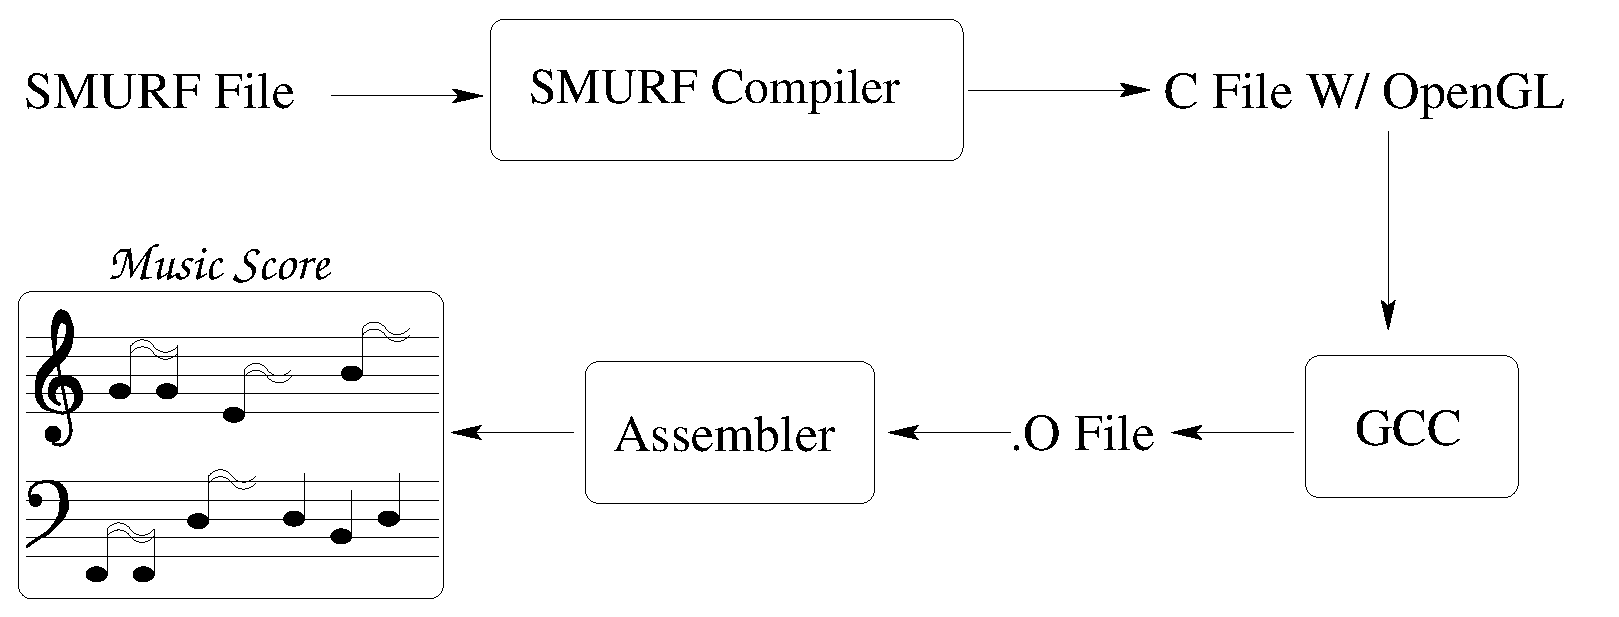
\includegraphics[width=0.75\textwidth]{figures/pipeline}
	\caption{SMURF pipeline for composing serialist music}
	\label{fig:pipeline}
\end{figure}

\section{Syntax}

SMURF is a functional programming language loosely modeled off of Haskell. It has immutable memory, no global variables and no I/O.

\subsection{Types}

\subsubsection{Standard Types}
\begin{itemize}
\item Integer: int
\item Boolean: bool
\item Tuples: elements can have different types
\item Lists: elements must have same type
\end{itemize}

\subsubsection{Note (pc: int, beat: int, register: int)}
\begin{itemize}
\item pc (pitch class): represented by integers 0-11
  \begin{itemize}
  \item Note with pc = -1 represents a rest, used in Measure type
  \end{itemize}
\item beat: represented by powers of 2 up to 32 (assuming \Takt{4}{4} time)
\item register: represented by integers -2 to 2
  \begin{itemize}
  \item \begin{music}  \trebleclef  \end{music}  Treble Clef: notes middle C and higher represented by 0-2  
  \item \begin{music} \bassclef  \end{music}  Bass Clef: notes lower than middle C represented by negative numbers
  \end{itemize}
\end{itemize}

\subsubsection{Chord ([Note])}
\begin{itemize}
\item Type checks that all notes have same beat count
\end{itemize}

\subsubsection{Measure ([Chord])}
\begin{itemize}
\item Type check that measure has exactly 4 beats
\end{itemize}

\subsubsection{Score ([Measure])}

\subsubsection{Functions}
A function is a type whose value can be defined with an expression
\begin{itemize}
\item Function declarations must declare type (can declare general type)
\item Function declarations must be on own line
\item No explicit return
\item Pattern matching, guards, and if-then-else clauses used
  \begin{itemize}
  \item Each pattern matching pattern must be on own line
  \item Guards and if-then-else clauses do not have newline restrictions
  \end{itemize}
\end{itemize}

\begin{table} [h]
	\centering
    \begin{tabular}{ll}
    \hline\hline
    Operators & \\
    \hline\hline
       \textbackslash n & End of line: Terminates phrases \\ \hline
      + & Integer arithmetic: plus  \\ \hline
      - & Integer arithmetic: minus  \\ \hline 
      \% & Integer arithmetic: modulus, ignores negatives  \\ \hline
      = & Assignment operator \\ \hline
      \textless  & Comparison \\ \hline
      \textgreater  & Comparison \\ \hline
      \textless=  & Comparison \\ \hline
      \textgreater= & Comparison \\ \hline
       == & Boolean operator: Structural comparison  \\ \hline
       not & Boolean operator \\ \hline
       \&\& & Boolean operator \\ \hline
       \textbar\textbar & Boolean operator \\ \hline
       \textbar & Boolean operator, used with guards\\ \hline
       :: & Type specification \\ \hline
       \textendash\textgreater & Argument and function return type specification  \\ \hline
      ++ & Concatenation: concat \\ \hline
      : & Construction: cons \\ \hline
      /* */ & Multiline comments, nesting allowed \\ \hline
      // & Single-line comment \\ \hline
    \end{tabular}
\end{table}

\begin{table} [h]
	\centering
    \begin{tabular}{ll}
    \hline\hline
    Keywords & \\ 
    \hline\hline
      let & Specify values and functions  \\ \hline
      in & Allow local variable binding in expression \\ \hline
      if, then, else & Specify conditional expression, else compulsory  \\ \hline
      gen\_score & Generate musical score given Score as argument  \\ \hline
    \end{tabular}
\end{table}


\section{Examples}

dummy contents...



% citations begin here
\bibliographystyle{ieeetr}
\bibliography{ref/refs}


\end{document}
